\documentclass[11pt,a4paper]{article}

% Core packages
\usepackage[utf8]{inputenc}
\usepackage[T1]{fontenc}
\usepackage{lmodern}
\usepackage{microtype}
\usepackage[margin=1in]{geometry}

% Bibliography
\usepackage[numbers,sort&compress]{natbib}

% Figures and tables
\usepackage{graphicx}
\usepackage{booktabs}
\usepackage{array}
\usepackage{multirow}

% TikZ
\usepackage{tikz}
\usepackage{pgfplots}
\pgfplotsset{compat=1.18}
\usetikzlibrary{arrows.meta,positioning,shapes.geometric,fit,backgrounds,calc,decorations.pathreplacing}

% Math
\usepackage{amsmath,amssymb,amsthm}

% Theorem environments
\newtheorem{definition}{Definition}
\newtheorem{theorem}{Theorem}
\newtheorem{lemma}[theorem]{Lemma}
\newtheorem{corollary}[theorem]{Corollary}
\newtheorem{proposition}[theorem]{Proposition}
\theoremstyle{definition}
\newtheorem{example}{Example}
\newtheorem{remark}{Remark}

% Links
\usepackage[colorlinks=true,linkcolor=blue,citecolor=blue,urlcolor=blue]{hyperref}

% Headers
\usepackage{fancyhdr}
\setlength{\headheight}{14pt}
\pagestyle{fancy}
\fancyhf{}
\rhead{\thepage}

% Author block
\usepackage{authblk}

\title{The Latency Floor of Cascade Voice Agents:\\
Formal Bounds and Design Levers}

\author[1,2]{Daniel Garc\'ia Pe\~na}
\affil[1]{Department of Energy and Process Control, University of Oviedo, Oviedo, Spain.}
\affil[2]{AI Engineering, Unicaja Bank, Spain.
  \texttt{info@iamdgarcia.com}}

\date{\today}

\begin{document}

\maketitle

\begin{abstract}
Voice-based conversational agents are built using two competing paradigms:
native audio models, which process speech end-to-end, and cascade architectures,
which chain speech recognition, a text language model, and speech synthesis in
series.
Cascade agents are cheaper, more auditable, and easier to equip with tools, but
suffer from a perceived silence gap between user utterance and agent response
that native models largely eliminate.
We present the first formal analysis of this gap.
We model the cascade pipeline as a directed acyclic graph of latency-contributing
stages and decompose each stage's latency into a reducible component, improvable
with faster models or hardware, and an irreducible component determined by
architectural structure.
We prove a \emph{Latency Floor Theorem}: the total silence gap has a lower bound
$\Lambda^*$ that no cascade architecture can cross without changing its topology.
We derive the \emph{Cascade Competitiveness Criterion}, the formal condition under
which a cascade agent achieves perceptual equivalence with a native voice model.
We extend the model to tool-using ReAct agents and prove that each reasoning step
compounds the silence gap by a full latency cycle, making competitiveness
increasingly unlikely for multi-step agents.
Finally, we classify six design levers --- streaming synthesis, barge-in
detection, filler generation, speculative decoding, parallel tool execution, and
hybrid routing --- by the latency component each addresses and the headroom each
recovers.
Our analysis gives practitioners a principled basis for choosing between cascade
and native voice architectures and for engineering cascade agents that approach
the perceptual quality of native systems.
\end{abstract}

\section{Introduction}
\label{sec:introduction}
% §1 Introduction
Voice-based conversational interfaces are increasingly deployed in real-world applications,
from customer service \citep{openai2024realtimeapi} to personal assistants \citep{google2024geminivoice}.
Two competing architectural paradigms have emerged for building such systems.
\emph{Native voice models} process speech end-to-end within a single neural network,
eliminating inter-component boundaries and their associated latencies.
\emph{Cascade architectures} decompose the pipeline into three sequential components:
a speech recognition model that transcribes user audio to text,
a text-based language model that reasons and generates a response,
and a speech synthesis model that renders the response as audio.

Cascade architectures offer compelling practical advantages.
They are substantially cheaper to operate than native voice APIs \citep{openai2024realtimeapi}.
They allow the language model component to be replaced or updated independently.
They support tool use---the ability to call external APIs, databases, and services---through
standard text-based agent frameworks \citep{yao2023react,langgraph2024}.
They expose intermediate representations (transcripts, structured outputs) that aid
auditability, debugging, and safety monitoring.

Despite these advantages, cascade architectures suffer from a perceptual deficiency:
the \emph{silence gap}.
When a user finishes speaking, the cascade pipeline must complete speech recognition,
then wait for the language model to produce its first token,
then wait for the speech synthesis model to begin audio playback.
The sum of these delays produces an interval of silence that users perceive as unnatural.
Human conversation tolerates gaps of roughly 200 milliseconds before perceiving a response
as delayed \citep{levinson2015timing,stivers2009universals}.
Cascade pipelines routinely exceed this threshold by a factor of four to ten.

This gap is widely acknowledged in the engineering literature as a key limitation of cascade
voice systems, but it has received no formal treatment.
Practitioners address it through ad hoc engineering mitigations without a principled basis
for understanding which strategies reduce the gap structurally and which merely mask it
perceptually.
No prior work has formally characterized the irreducible latency floor of cascade voice pipelines as a function of pipeline topology, nor established formal conditions under which such systems can approach human conversational response norms.

This paper provides that framework.
We introduce the \emph{turn-taking threshold} $\tau_{human} = 200$~ms as the upper bound on
the \emph{silence gap}---the interval of silence between the end of the user's utterance and
the beginning of the agent's audio response---within which a \emph{cascade architecture} is
perceived as conversationally natural.
We make the following contributions:

\begin{enumerate}
\item \textbf{Formal pipeline model} (\S\ref{sec:pipeline_model}).
We represent the cascade voice pipeline as a directed acyclic graph of latency-contributing
stages and decompose each stage's latency into a \emph{reducible} component,
improvable with faster models or hardware, and an \emph{irreducible} component,
determined by architectural structure and eliminable only by changing the pipeline topology.

\item \textbf{Latency Floor Theorem} (\S\ref{sec:latency_floor}).
We prove that the silence gap of any cascade architecture has a lower bound $\Lambda^*$,
the sum of irreducible latencies across all pipeline stages,
that cannot be reduced by any model improvement or hardware upgrade.
We derive the \emph{Cascade Competitiveness Criterion} (CCC),
the formal condition under which a cascade architecture achieves perceptual equivalence
with a native voice model.

\item \textbf{ReAct extension} (\S\ref{sec:react_extension}).
We extend the formal model to tool-using agents built on the ReAct pattern \citep{yao2023react}.
We prove that each reasoning step adds a full latency cycle to the silence gap,
compounding the irreducible floor and making CCC satisfaction increasingly unlikely
for multi-step agents.

\item \textbf{Design lever taxonomy} (\S\ref{sec:design_levers}).
We classify six mitigation strategies by the latency component each targets,
the headroom each can recover, and its side effects.
We show that only two strategies---streaming synthesis and hybrid routing---reduce
the irreducible floor $\Lambda^*$ itself;
the remaining four are perceptual patches that mask the gap without reducing it.

\item \textbf{Open problems} (\S\ref{sec:open_problems}).
We identify four open research directions emerging from the formal analysis:
learned barge-in prediction, safety in cascade voice systems,
voice-aware agent planning, and principled hybrid routing policies.
\end{enumerate}

The remainder of this paper is organised as follows.
Section~\ref{sec:background} introduces the cascade pipeline architecture,
native voice models, and human turn-taking thresholds.
Section~\ref{sec:pipeline_model} develops the formal model.
Sections~\ref{sec:latency_floor} and~\ref{sec:react_extension} state and prove the main theorems.
Section~\ref{sec:design_levers} presents the design lever taxonomy.
Sections~\ref{sec:open_problems} and~\ref{sec:discussion} discuss implications.
Section~\ref{sec:conclusion} concludes.


\section{Background}
\label{sec:background}
% §2 Background
\subsection{Cascade Voice Architectures}

A cascade voice architecture chains three independently developed components.

\paragraph{Speech recognition.}
The \emph{automatic speech recognition} (ASR) component converts raw audio input to text.
Modern ASR systems are based on encoder-decoder transformers \citep{radford2022whisper}
or connectionist temporal classification models \citep{graves2006ctc}.
ASR latency has two subcomponents:
\emph{buffering latency}, the time required to accumulate sufficient audio before decoding begins,
which is determined by the end-of-utterance detection (VAD) threshold and cannot be reduced below
the duration of the final word or phrase of the user's turn,
and \emph{decoding latency}, the time to run the recognition model on the buffered audio,
which is reducible with faster hardware or smaller models.
Voice activity detection systems \citep{raux2008optimizing} trigger the end-of-utterance signal
that releases the audio buffer to the ASR model.
The VAD threshold is a critical parameter: a low threshold reduces buffering latency but
increases the rate of premature cut-offs, while a high threshold increases buffering latency
but improves transcription accuracy.
Specaugment \citep{park2019specaugment} and related data augmentation techniques improve
ASR robustness without affecting the latency decomposition.

\paragraph{Language model.}
The language model (LM) component receives the ASR transcript as text input and produces a
text response.
\emph{First-token latency} (also called time-to-first-token, TTFT) is the delay between the LM
receiving input and emitting its first output token.
TTFT is determined by the time to prefill the model's key-value cache with the input context.
For autoregressive transformers \citep{vaswani2017attention}, this is linear in context length
and quadratic in sequence length for self-attention.
Subsequent token generation proceeds at a rate determined by memory bandwidth,
not compute \citep{leviathan2023fast}.
The LM is the only cascade stage that performs open-ended reasoning;
all other stages perform fixed-function transformations.

\paragraph{Speech synthesis.}
The \emph{text-to-speech} (TTS) component converts the LM's text output to audio.
Classic systems such as Tacotron~2 \citep{shen2018natural} and WaveNet \citep{oord2016wavenet}
generate audio non-autoregressively from a complete text input.
Streaming TTS systems can begin audio generation after receiving a short initial text segment,
reducing the time before audio playback begins at the cost of potentially lower quality
for very short prefixes.
The first audio chunk emitted by the TTS model must reach the playback buffer before the
user hears any agent speech;
this buffering delay is part of the irreducible floor when the TTS model cannot begin
synthesis without a minimum text prefix.

\paragraph{Total silence gap.}
The total silence gap in a cascade architecture is the time from the end of the user's utterance
to the beginning of the agent's audio response.
Under the standard (non-streaming) cascade configuration, this equals the sum of:
ASR buffering latency, ASR decoding latency, LM first-token latency, and TTS initial audio latency.
We refer to this sum as the \emph{silence gap} throughout this paper.
The cascade architecture is distinguished from alternative designs precisely by the fact that
these four components contribute additively and sequentially to the silence gap.

\subsection{Native Voice Models}

Native voice models process speech input and produce speech output within a single end-to-end
neural network, eliminating the inter-component boundaries present in cascade architectures.
The key structural difference is that native models can begin producing audio output before
all input audio has been received, enabling sub-200~ms response latencies under favourable
network conditions.

OpenAI's Realtime API \citep{openai2024realtimeapi} exposes a GPT-4o variant that accepts
audio input and produces audio output directly via a WebSocket connection,
with reported response latencies of 320--500~ms.
Google's Gemini Live \citep{google2024geminivoice} provides a similar capability
with streaming audio input and output.
Both systems represent the current state of the art for low-latency voice interaction.

Native voice models eliminate ASR and TTS as separate stages.
They process audio tokens directly, enabling the model to begin generating audio
before the user has finished speaking and to detect barge-in events internally.
The latency of a native voice model is therefore dominated by the time from receiving
sufficient audio context to emitting the first audio output token,
which is bounded below by the model's forward pass time on the input context.

Native voice models support function calling in audio mode~\citep{openai2024realtimeapi};
however, tool-call turns require the model to pause audio generation while the external tool executes,
partially reintroducing sequential latency that increases with the number of tool calls.
This characteristic makes native voice models less suited for applications requiring
real-time access to databases, APIs, or other external services with non-trivial round-trip latency.
Cascade architectures retain a structural advantage for auditable, tool-intensive applications,
motivating the analysis in this paper.

\subsection{Human Turn-Taking and Perceptual Thresholds}

Human conversation is governed by tight timing constraints.
\citet{levinson2015timing} report that the modal inter-turn interval in natural conversation
is approximately 0~ms (overlapping speech) to 200~ms across typologically diverse languages.
\citet{stivers2009universals} confirm this finding across ten unrelated languages,
establishing the 200~ms threshold as a near-universal feature of human turn-taking.
Response gaps exceeding 700--800~ms are perceived as face-threatening or indicative of
uncertainty \citep{levinson2015timing}.
These findings have been replicated in laboratory settings with synthesised speech,
suggesting that the perceptual threshold applies to machine voices as well as human voices.

We adopt $\tau_{human} = 200$~ms as the upper bound on the silence gap within which a voice
agent is perceived as conversationally natural.
We note that this threshold is context-dependent:
task-oriented dialogue (e.g., information retrieval) tolerates longer gaps than casual conversation,
and individual users vary in their sensitivity.
Our formal analysis treats $\tau_{human}$ as a parameter; the 200~ms value is used in worked
examples.
The term \emph{turn-taking threshold} $\tau_{human}$ is used throughout this paper to refer
to this perceptual boundary.

\subsection{Tool-Using Agents and the ReAct Pattern}

The ReAct pattern \citep{yao2023react} interleaves \emph{reasoning} steps, in which the language
model generates a chain-of-thought, with \emph{acting} steps, in which the model calls an
external tool and observes its result.
A $k$-step ReAct agent executes $k$ reasoning--action cycles before producing its final response.
This pattern improves task completion rates on multi-step reasoning benchmarks
but introduces additional latency before the agent can begin its final response.

In voice deployments, ReAct agents are typically implemented using structured output generation:
each LM inference step produces either a \texttt{tool\_call} action (with arguments) or a
\texttt{message} action (the final response to the user).
Frameworks such as LangGraph \citep{langgraph2024} orchestrate these cycles,
routing tool call results back to the LM as observations.
Each cycle adds a full LM inference pass (prefill + decode) and a tool execution round-trip to the
silence gap before the user hears any audio response.
Chain-of-thought reasoning \citep{wei2023chainofthought} improves response quality but
further increases TTFT by extending the generated sequence before the final answer token.
The compounding effect of multiple ReAct cycles on the silence gap is one of the central
analytical results of this paper, developed formally in Section~\ref{sec:react_extension}.
Recent work on voice agent system design \citep{dong2024building} identifies multi-step
tool use as a primary source of perceived latency in deployed cascade voice agents,
motivating the formal treatment we provide here.

\subsection{Spoken Dialogue Systems and Incremental Processing}

The spoken dialogue systems (SDS) community has long studied the sequential latency accumulation problem in cascade speech pipelines~\citep{schlangen2011general,skantze2021turn}.
\citet{schlangen2011general} introduce a general formal model of incremental dialogue processing in which each module produces output incrementally, motivating overlap between pipeline stages as the primary mechanism for latency reduction.
\citet{skantze2021turn} survey turn-taking in conversational systems and human-robot interaction, providing an engineering-facing bridge between psycholinguistic turn-taking norms and deployed dialogue system timing.
\citet{raux2008optimizing} demonstrate empirically how end-of-utterance threshold configuration affects perceived response latency in deployed voice systems.
Our work is distinguished from this literature by deriving a formal lower bound on the irreducible latency floor as a function of pipeline topology, and by connecting this bound explicitly to the human conversational gap tolerance threshold and to multi-step tool-using agents.


\section{Formal Pipeline Model}
\label{sec:pipeline_model}
% §3 Formal Pipeline Model
We develop a formal model of the cascade voice pipeline that separates
structurally removable latency from latency imposed by the pipeline topology.

\subsection{Stages and the Pipeline DAG}

\begin{definition}[Pipeline Stage]
A \emph{pipeline stage} $s_i$ is a computational unit that receives a discrete input
$x_i$ and produces a discrete output $y_i = f_i(x_i)$ after a latency of
$\lambda_i(x_i) \geq 0$ seconds, where $\lambda_i$ may depend on the input.
\end{definition}

\begin{definition}[Cascade Pipeline DAG]
\label{def:cascade_dag}
A \emph{cascade pipeline} is a directed acyclic graph $G = (S, E)$ where
$S = \{s_1, \ldots, s_n\}$ is a set of pipeline stages and
$E \subseteq S \times S$ is a set of dependency edges.
An edge $(s_i, s_j) \in E$ indicates that $s_j$ cannot begin execution until $s_i$
has produced its complete output.
The standard cascade voice pipeline has $S = \{s_{asr}, s_{lm}, s_{tts}\}$ and
edges $E = \{(s_{asr}, s_{lm}), (s_{lm}, s_{tts})\}$, forming a linear chain.
\end{definition}

\begin{definition}[EOU-Gated Cascade (EGC)]
\label{def:egc}
A cascade pipeline $G$ is \emph{EOU-gated} if:
(a)~$s_{asr}$ begins decoding only after an end-of-utterance signal is confirmed;
(b)~no stage $s_j$ begins execution until its predecessor $s_{j-1}$ has produced its
complete output; and
(c)~all stage execution occurs in the post-speech interval $[0, \infty)$,
where $t = 0$ denotes the EOU event.
Theorems~\ref{thm:latency_floor} and~\ref{thm:react} and
Corollary~\ref{cor:impossibility} apply to EGC pipelines.
\end{definition}

\begin{definition}[Streaming Cascade (SC)]
\label{def:sc}
A cascade pipeline $G$ is a \emph{streaming cascade} if:
(a)~$s_{asr}$ produces a sequence of incrementally committed partial transcripts
$\{C_{pre}(t) : t \in [-T_{speech}, 0]\}$ during the user utterance of duration
$T_{speech}$, where $C_{pre}(t) \subseteq C_{full}$ for all $t$;
(b)~$s_{lm}$ may begin prefilling its key-value cache on $C_{pre}(t)$ at any
$t < 0$ (during speech); and
(c)~the EOU event at $t = 0$ releases $s_{lm}$ to begin its decode phase, which
cannot start before $t = 0$.
The \emph{residual context} $C_{residual} = C_{full} \setminus C_{pre}(0^-)$
is the set of tokens whose prefill must occur post-EOU.
The \emph{commit latency} $\delta_N$ is the delay between EOU and the moment
$C_{full}$ is finalised by $s_{asr}$.
\end{definition}

\subsection{Reducible and Irreducible Latency}

\begin{definition}[Reducible and Irreducible Latency]
\label{def:decomposition}
The latency of stage $s_i$ decomposes as:
\begin{equation}
  \lambda_i = \lambda_i^r + \lambda_i^{irr}
\end{equation}
where $\lambda_i^{irr}$ is defined as the infimum of $\lambda_i$ over all valid implementations of stage $s_i$:
\begin{equation}
  \lambda_i^{irr} := \inf_{\mathcal{I} \in \mathrm{valid}(s_i)} \lambda_i^{\mathcal{I}}
\end{equation}
A \emph{valid implementation} $\mathcal{I} \in \mathrm{valid}(s_i)$ is any choice of model weights, inference hardware, and serving configuration that preserves the stage's required input--output contract (i.e., the same mapping $x_i \mapsto y_i = f_i(x_i)$ is computed, up to equivalent quality).
The \emph{reducible} component $\lambda_i^r := \lambda_i - \lambda_i^{irr} \geq 0$ is the gap between the current implementation's latency and this infimum.
\end{definition}

We characterise $\lambda_i^{irr}$ for each stage of the standard cascade pipeline.

\paragraph{ASR irreducible latency.}
Under the EOU-gated cascade (Definition~\ref{def:egc}), the ASR stage must buffer audio
until end-of-utterance is detected before transcription can begin.
Let $d_{eou}$ denote the duration of the end-of-utterance detector's analysis window.
Then $\lambda_{asr}^{irr} \geq d_{eou}$, since no transcription can begin before the
detector confirms the user has stopped speaking.
For voice activity detection systems operating on 30~ms frames \citep{raux2008optimizing},
$d_{eou}$ is typically 200--600~ms.
Under the streaming cascade (Definition~\ref{def:sc}), $\lambda_{asr}^{irr}$ is replaced
by the commit latency $\delta_N$ of the final word from EOU;
for streaming RNN-T systems \citep{sainath2020streaming} $\delta_N \approx 150$--320~ms,
which is strictly smaller than $d_{eou}$ for typical VAD thresholds.
The Latency Floor Theorem and Impossibility Corollary (Section~\ref{sec:latency_floor})
are stated for the EGC model; Section~\ref{sec:latency_floor} also derives the floor for SC.

\paragraph{LM irreducible latency.}
A transformer language model \citep{vaswani2017attention} must compute the prefill
key-value cache over its full input context before generating the first output token.
Let $|C|$ denote context length in tokens and $\alpha$ the per-token prefill cost.
Then $\lambda_{lm}^{irr} \geq \alpha \cdot |C|$.
This cost is architectural: it cannot be eliminated without changing the attention
mechanism or the requirement to condition on the full context.

\paragraph{TTS irreducible latency.}
A TTS system must process at least a minimum text prefix
before audio playback can begin.
For autoregressive synthesis, this is the time to generate the first audio frame
from the first input token.
For non-streaming systems \citep{shen2018natural}, the entire text must be generated first,
giving a much larger $\lambda_{tts}^{irr}$.

\subsection{The Silence Gap}

\begin{definition}[Silence Gap]
\label{def:silence_gap}
The \emph{silence gap} $\Lambda$ of a cascade pipeline is the elapsed time between
the end of the user's utterance and the beginning of the agent's audio response.
For a linear cascade pipeline with stages $s_{asr}, s_{lm}, s_{tts}$:
\begin{equation}
  \Lambda = \lambda_{asr} + \lambda_{lm} + \lambda_{tts}
          = \sum_{i \in \{asr, lm, tts\}} (\lambda_i^r + \lambda_i^{irr})
\end{equation}
\end{definition}

Figure~\ref{fig:pipeline_dag} illustrates the pipeline DAG and the decomposition of
each stage's latency into reducible and irreducible components.

\begin{figure}[t]
  \centering
  \resizebox{\linewidth}{!}{%
    % Fig 1: Cascade pipeline DAG with reducible/irreducible latency annotations
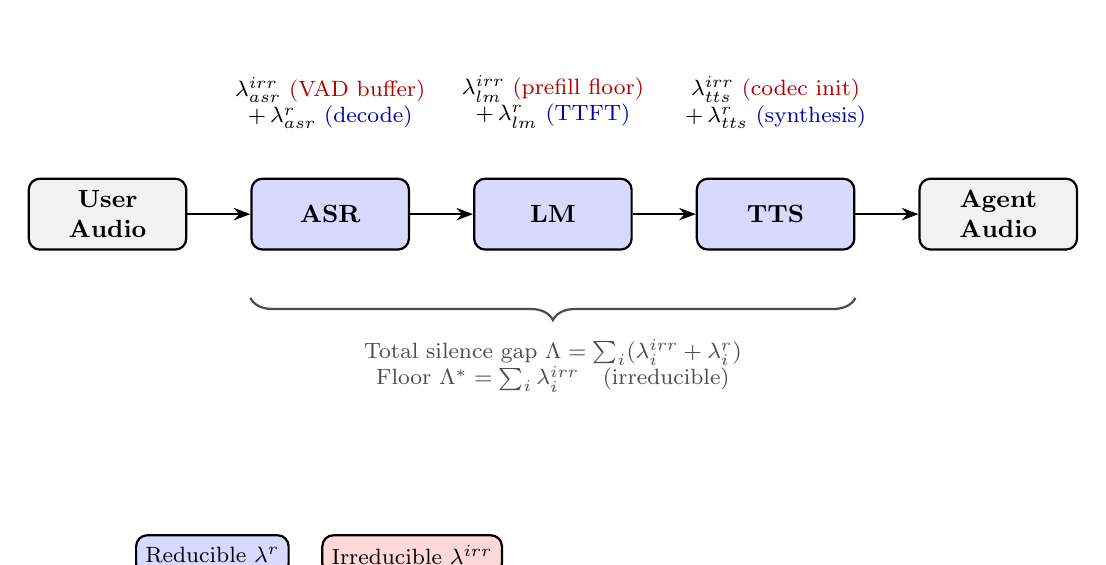
\begin{tikzpicture}[
  node distance=1.4cm and 0.8cm,
  box/.style={rectangle, rounded corners=4pt, draw=black, thick,
              minimum width=2.0cm, minimum height=0.9cm,
              font=\small\bfseries, align=center},
  reducible/.style={fill=blue!15},
  irreducible/.style={fill=red!15},
  arr/.style={-{Stealth[length=6pt]}, thick},
  annot/.style={font=\footnotesize, align=center}
]

% Nodes
\node[box, fill=gray!10] (user) {User\\Audio};
\node[box, reducible,  right=of user]  (asr)  {ASR};
\node[box, reducible,  right=of asr]   (lm)   {LM};
\node[box, reducible,  right=of lm]    (tts)  {TTS};
\node[box, fill=gray!10, right=of tts] (out)  {Agent\\Audio};

% Arrows
\draw[arr] (user) -- (asr);
\draw[arr] (asr)  -- (lm);
\draw[arr] (lm)   -- (tts);
\draw[arr] (tts)  -- (out);

% Latency annotations above each stage
\node[annot, above=0.5cm of asr] (lasr)
  {$\lambda_{asr}^{irr}$ \textcolor{red!70!black}{(VAD buffer)}\\
   $+\,\lambda_{asr}^{r}$ \textcolor{blue!70!black}{(decode)}};
\node[annot, above=0.5cm of lm]  (llm)
  {$\lambda_{lm}^{irr}$ \textcolor{red!70!black}{(prefill floor)}\\
   $+\,\lambda_{lm}^{r}$ \textcolor{blue!70!black}{(TTFT)}};
\node[annot, above=0.5cm of tts] (ltts)
  {$\lambda_{tts}^{irr}$ \textcolor{red!70!black}{(codec init)}\\
   $+\,\lambda_{tts}^{r}$ \textcolor{blue!70!black}{(synthesis)}};

% Brace below showing total silence gap
\draw[decorate, decoration={brace, amplitude=8pt, mirror},
      thick, color=black!70]
  ([yshift=-0.6cm]asr.south west) -- ([yshift=-0.6cm]tts.south east)
  node[midway, below=0.4cm, annot]
  {Total silence gap $\Lambda = \sum_i (\lambda_i^{irr} + \lambda_i^r)$\\
   Floor $\Lambda^* = \sum_i \lambda_i^{irr}$\quad (irreducible)};

% Legend — placed below the brace label to avoid overlap
\node[box, reducible, below left=3.6cm and -0.5cm of asr,
      minimum width=1.8cm, minimum height=0.5cm, font=\footnotesize]
  (leg_r) {Reducible $\lambda^r$};
\node[box, irreducible, right=0.4cm of leg_r,
      minimum width=1.8cm, minimum height=0.5cm, font=\footnotesize]
  (leg_i) {Irreducible $\lambda^{irr}$};

\end{tikzpicture}
%
  }
  \caption{The cascade voice pipeline as a directed acyclic graph.
           Each stage's latency decomposes into a reducible component
           (blue, improvable with faster models) and an irreducible component
           (red, structurally determined).
           The total silence gap $\Lambda$ spans all three stages;
           its irreducible floor $\Lambda^*$ cannot be reduced without
           changing the pipeline topology.}
  \label{fig:pipeline_dag}
\end{figure}

\subsection{Worked Example}

Table~\ref{tab:latency_example} provides representative latency values for a
typical cloud-hosted cascade pipeline based on published and empirically observed figures.

\begin{table}[t]
  \centering
  \caption{Representative latency decomposition for a cloud-hosted cascade pipeline.
           Reducible values reflect current best-in-class implementations;
           irreducible values are architectural lower bounds.
           Values are representative estimates based on published benchmarks \citep{radford2022whisper,oord2016wavenet,vaswani2017attention}; empirical ranges vary by hardware, model size, and serving infrastructure.
           The LM irreducible value of 100~ms assumes optimised serving on high-end hardware and is intended as the floor for the formal analysis, not a guaranteed real-world value.}
  \label{tab:latency_example}
  \begin{tabular}{lrrrr}
    \toprule
    Stage & $\lambda_i^{irr}$ (ms) & $\lambda_i^r$ (ms) & $\lambda_i$ (ms) \\
    \midrule
    ASR (Whisper-class \citep{radford2022whisper})  & 200  & 150 & 350 \\
    LM  (GPT-4o-class, 8k context)                  & 100  & 250 & 350 \\
    TTS (streaming synthesis)                        & 80   & 120 & 200 \\
    \midrule
    \textbf{Total}                                   & \textbf{380} & \textbf{520} & \textbf{900} \\
    \bottomrule
  \end{tabular}
\end{table}

In this example, the silence gap is 900~ms --- approximately 4.5$\times$ the human
turn-taking threshold $\tau_{human} = 200$~ms.
Even with infinitely fast reducible components ($\lambda_i^r \to 0$),
the irreducible floor $\Lambda^* = 380$~ms remains nearly twice $\tau_{human}$.


\section{The Latency Floor Theorem}
\label{sec:latency_floor}
% §4 The Latency Floor Theorem
We now prove the central result: the silence gap of any cascade pipeline has an
irreducible lower bound.

\subsection{The Latency Floor Theorem}

\begin{theorem}[Latency Floor]
\label{thm:latency_floor}
Let $G = (S, E)$ be an \emph{EOU-gated cascade} (Definition~\ref{def:egc}) with stages
$S = \{s_1, \ldots, s_n\}$ forming a linear chain.
Let each stage $s_i$ have latency decomposed as $\lambda_i = \lambda_i^r + \lambda_i^{irr}$
per Definition~\ref{def:decomposition}.
The following premises are assumed:
\begin{enumerate}
  \item \emph{Sequential execution}: stages execute strictly sequentially; no stage begins
        processing before its predecessor has produced its complete output.
        (This premise holds by definition for EGC; it does \emph{not} hold for the streaming
        cascade of Definition~\ref{def:sc}, which is analysed separately in
        Theorem~\ref{thm:streaming_floor}.)
  \item \emph{Input independence}: each stage latency $\lambda_i$ is treated as independent of the specific input $x_i$ (a simplifying assumption acknowledged in Section~\ref{sec:discussion}).
  \item \emph{Implementation}: an ``implementation'' of $G$ is any choice of model weights, inference hardware, and serving configuration that preserves the pipeline topology and stage boundary definitions; the set of valid implementations for each stage is $\mathrm{valid}(s_i)$ as defined in Definition~\ref{def:decomposition}.
\end{enumerate}
Then the silence gap satisfies:
\begin{equation}
  \Lambda \geq \Lambda^* := \sum_{i=1}^{n} \lambda_i^{irr}
\end{equation}
for all implementations of $G$, regardless of model size, hardware, or inference optimisation.
\end{theorem}

\begin{proof}
Each stage $s_j$ in the linear chain cannot begin execution until $s_{j-1}$ produces its output,
by Definition~\ref{def:cascade_dag} (Cascade Pipeline DAG).
Therefore the silence gap is at least the sum of the first-output latencies of all stages:
$\Lambda \geq \sum_i \lambda_i$.
Since $\lambda_i = \lambda_i^r + \lambda_i^{irr}$ and $\lambda_i^r \geq 0$,
we have $\Lambda \geq \sum_i \lambda_i^{irr} = \Lambda^*$.
The reducible terms $\lambda_i^r$ can be made arbitrarily small by using faster models
(in the limit of infinite compute), but $\lambda_i^{irr}$ is by definition the lower bound
achievable for any implementation of $s_i$ given its input--output contract.
Therefore $\Lambda^*$ is a lower bound on $\Lambda$ for any cascade pipeline with topology $G$.
\end{proof}

\begin{remark}
Theorem~\ref{thm:latency_floor} applies to any linear or branching DAG topology.
For a branching pipeline where parallel stages can execute concurrently,
$\Lambda^*$ is the maximum irreducible latency along any critical path through the DAG,
not the sum over all stages.
The standard cascade pipeline is a single critical path,
so the sum form applies directly.
\end{remark}

\subsection{Native Voice as the Zero-Floor Limit}

A native voice model collapses the three-stage cascade into a single stage $s_{native}$
that maps audio input directly to audio output, eliminating inter-stage buffering latency.
Two architecturally distinct classes exist, with different prefill-hiding properties.

\paragraph{Buffer-and-commit (GPT-4o Realtime class).}
Systems such as GPT-4o Realtime \citep{openai2024realtimeapi} and Gemini Live
\citep{google2024geminivoice} stream audio into a server-side buffer during the user's speech.
VAD monitors the stream and, upon detecting end-of-utterance, commits the buffer and triggers
model inference.
The full audio-token prefill therefore begins \emph{after} EOU, analogously to EGC cascade:
\begin{equation}
  \Lambda^*_{RT,commit} = d_{eou}^{vad} + \alpha_{audio} \cdot N_{speech} + \lambda_{decode,1}
\end{equation}
The advantage over cascade is the elimination of the separate ASR decode and TTS stages,
not prefill hiding during speech.
Observed silence gaps of 320--500~ms are consistent with this structure.

\paragraph{Streaming causal (Moshi class).}
Systems such as Moshi \citep{defossez2024moshi} use a fully causal audio codec
(frame stride $\Delta_t = 80$~ms) and process each codec frame through the Temporal Transformer
as it arrives.
The KV cache grows continuously during the user's utterance:
by the time speech ends, the model has already prefilled all speech frames.
The post-EOU silence gap is therefore:
\begin{equation}
  \Lambda^*_{RT,stream} = \Delta_t + \lambda_{forward}^{(1)}
\end{equation}
where $\lambda_{forward}^{(1)}$ is the time for one Transformer step over the current KV state.
This gives a theoretical floor of approximately 160~ms, independent of utterance length.
The prefill advantage relative to EGC cascade is:
\begin{equation}
  \Lambda^*_{EGC} - \Lambda^*_{RT,stream}
    = \underbrace{\lambda_{asr}^{irr} + \lambda_{tts}^{irr}}_{\text{stage elimination}}
    + \underbrace{\alpha_{audio} \cdot N_{speech} - \lambda_{forward}^{(1)} - \Delta_t}_{\text{prefill hidden during speech}}
\end{equation}
The prefill-hiding term grows with utterance duration $T_{speech}$,
so streaming causal models gain a larger advantage for longer utterances.

The formal inequality chain is:
\begin{equation}
  \Lambda^*_{RT,stream} \leq \Lambda^*_{RT,commit} \leq \Lambda^*_{EGC}
\end{equation}
where the first gap reflects prefill hiding during speech and the second reflects
ASR and TTS stage elimination.
The paper's impossibility result (Corollary~\ref{cor:impossibility}) applies only to EGC cascade,
not to streaming cascade or native voice architectures.

\subsection{The Cascade Competitiveness Criterion}

\begin{definition}[Cascade Competitiveness Criterion]
\label{def:ccc}
A cascade pipeline is \emph{perceptually competitive} with a native voice model if and only if:
\begin{equation}
  \Lambda \leq \tau_{human}
\end{equation}
where $\tau_{human}$ is the human turn-taking threshold (approximately 200~ms,
as established by \citet{levinson2015timing} and \citet{stivers2009universals}).
\end{definition}

\begin{corollary}[Impossibility of Cascade Competitiveness]
\label{cor:impossibility}
If $\Lambda^* > \tau_{human}$, then no \emph{EOU-gated cascade} pipeline with topology $G$
can satisfy the Cascade Competitiveness Criterion, regardless of model or hardware improvements.
\end{corollary}

\begin{proof}
By Theorem~\ref{thm:latency_floor}, $\Lambda \geq \Lambda^*$.
If $\Lambda^* > \tau_{human}$, then $\Lambda > \tau_{human}$ for all implementations,
so the CCC $\Lambda \leq \tau_{human}$ cannot be satisfied.
\end{proof}

\begin{remark}
Corollary~\ref{cor:impossibility} is scoped to EOU-gated cascade.
Streaming cascade (Definition~\ref{def:sc}) violates premise~(1) of Theorem~\ref{thm:latency_floor}
by design, and therefore has a strictly lower latency floor, derived in Theorem~\ref{thm:streaming_floor} below.
\end{remark}

\begin{theorem}[Streaming Cascade Floor]
\label{thm:streaming_floor}
Let $G$ be a streaming cascade (Definition~\ref{def:sc}).
Let $\delta_N$ be the commit latency of the final word from EOU,
$\alpha$ the per-token LM prefill cost,
$|C_{residual}|$ the number of tokens not yet prefilled at EOU,
$\lambda_{lm}^{decode,irr}$ the time to generate the first output token from a
completed KV cache, and $\lambda_{tts}^{irr}$ the TTS irreducible latency.
Then:
\begin{equation}
  \Lambda_{SC} \geq \Lambda^*_{SC}
    := \delta_N + \alpha \cdot |C_{residual}| + \lambda_{lm}^{decode,irr} + \lambda_{tts}^{irr}
\end{equation}
The gain over the EGC floor is the prefill work amortised over the user's speech duration:
\begin{equation}
  \Lambda^*_{EGC} - \Lambda^*_{SC}
    = \alpha \cdot (|C_{user}| - |C_{residual}|)
    = \alpha \cdot |C_{pre}|
\end{equation}
where $|C_{pre}|$ is the number of tokens stably committed and prefilled during speech.
\end{theorem}

\begin{proof}
At $t = 0$ (EOU): (1)~$\delta_N$ has elapsed for the ASR to commit the final word; (2)~the
LM decode phase cannot begin before EOU by Definition~\ref{def:sc}(c); (3)~the residual
$\alpha \cdot |C_{residual}|$ tokens must be prefilled before the first output token is generated;
(4)~TTS cannot begin before the first LM output token.
Each term is irreducible under its respective stage contract.
The gain $\alpha \cdot |C_{pre}|$ is bounded above by $\lambda_{lm}^{irr}$ (the full EGC
prefill cost) and approaches zero as $T_{speech} \to 0$ (short utterances leave no time for overlap).
\end{proof}

\begin{corollary}[Streaming CCC Satisfiability]
\label{cor:streaming_ccc}
A streaming cascade can satisfy the Cascade Competitiveness Criterion if and only if:
\begin{equation}
  \delta_N + \lambda_{lm}^{decode,irr} + \lambda_{tts}^{irr} \leq \tau_{human}
\end{equation}
Substituting representative values ($\lambda_{lm}^{decode,irr} \approx 20$~ms,
$\lambda_{tts}^{irr} \approx 80$~ms, $\tau_{human} = 200$~ms), this requires
$\delta_N \leq 100$~ms.
Streaming RNN-T systems \citep{sainath2020streaming} achieve $\delta_N \approx 150$--320~ms
at production accuracy, placing the CCC at the boundary of feasibility.
Fully causal CTC architectures with minimal lookahead can achieve $\delta_N \approx 100$~ms
at a 5--15\% relative word error rate cost \citep{yao2021wenet}.
\end{corollary}

Figure~\ref{fig:perceptual_threshold} illustrates the relationship between
the latency floor $\Lambda^*$, the total silence gap $\Lambda$, and the human threshold.

\begin{figure}[t]
  \centering
  \resizebox{\linewidth}{!}{%
    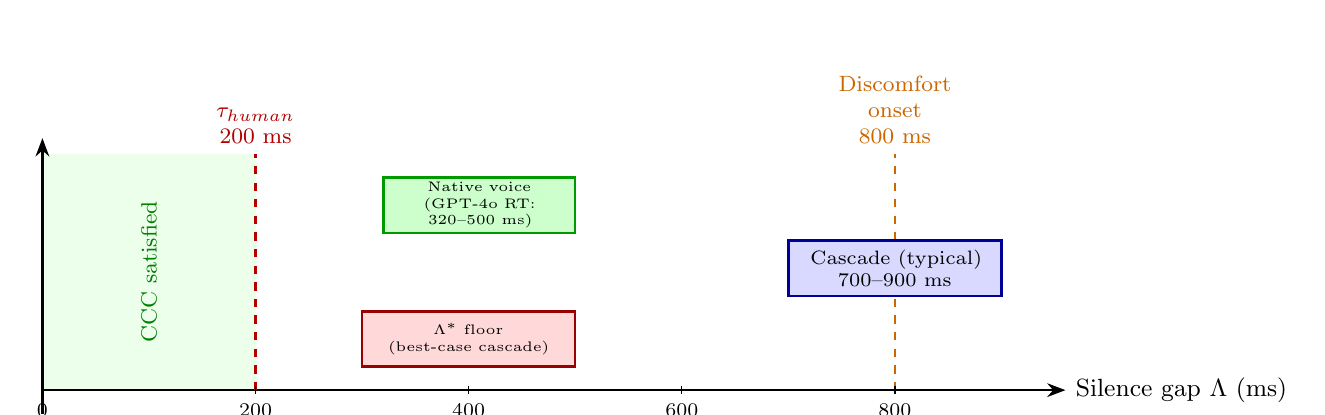
\begin{tikzpicture}[x=0.01354cm, y=1cm]

% CCC satisfied zone (green background)
\fill[green!8] (0,0) rectangle (200,3);

% Axis
\draw[-{Stealth}, thick] (0,0) -- (960,0)
  node[right, font=\small] {Silence gap $\Lambda$ (ms)};
\draw[-{Stealth}, thick] (0,-0.3) -- (0,3.2);

% Threshold markers
\draw[dashed, thick, red!70!black] (200,0) -- (200,3)
  node[above, font=\footnotesize, align=center] {$\tau_{human}$\\200 ms};
\draw[dashed, thick, orange!80!black] (800,0) -- (800,3)
  node[above, font=\footnotesize, align=center] {Discomfort\\onset\\800 ms};

% Native voice band (320--500 ms; lies entirely outside the CCC zone)
\fill[green!20] (320,2.0) rectangle (500,2.7);
\draw[green!60!black, thick] (320,2.0) rectangle (500,2.7);
\node[font=\tiny, align=center, text width=2.4cm] at (410,2.35)
  {Native voice\\(GPT-4o RT: 320--500 ms)};

% Cascade optimised band
\fill[blue!15] (700,1.2) rectangle (900,1.9);
\draw[blue!60!black, thick] (700,1.2) rectangle (900,1.9);
\node[font=\scriptsize, align=center, text width=2.6cm] at (800,1.55)
  {Cascade (typical)\\700--900 ms};

% Cascade floor band
\fill[red!15] (300,0.3) rectangle (500,1.0);
\draw[red!60!black, thick] (300,0.3) rectangle (500,1.0);
\node[font=\tiny, align=center, text width=2.2cm] at (400,0.65)
  {$\Lambda^*$ floor\\(best-case cascade)};

% CCC zone label (rotated)
\node[font=\footnotesize, color=green!50!black, rotate=90] at (100,1.5)
  {CCC satisfied};

% x-axis ticks
\foreach \x in {0,200,400,600,800} {
  \draw (\x, 0.05) -- (\x, -0.05)
    node[below, font=\scriptsize] {\x};
}

\end{tikzpicture}
%
  }
  \caption{Perceptual threshold diagram.
           The green zone ($\Lambda \leq \tau_{human} = 200$~ms) is the region where
           the Cascade Competitiveness Criterion is satisfied.
           Buffer-and-commit native voice models such as GPT-4o Realtime (green band,
           320--500~ms) fall outside the strict 200~ms CCC zone, yet are substantially
           below typical cascade latency.
           A typical cascade pipeline (blue band) operates well beyond it.
           The best-case cascade floor $\Lambda^*$ (red band) remains above
           $\tau_{human}$, establishing the impossibility result of
           Corollary~\ref{cor:impossibility}.}
  \label{fig:perceptual_threshold}
\end{figure}

\subsection{Practical Interpretation of \texorpdfstring{$\tau_{human}$}{tau\_human}}

The threshold $\tau_{human} = 200$~ms is derived from the modal inter-turn interval observed in human-human conversation \citep{levinson2015timing,stivers2009universals}.
We note that human tolerance for machine voices is empirically somewhat higher than for human interlocutors: users of voice assistants typically accept gaps up to 300--500~ms without explicit dissatisfaction \citep{levinson2015timing}.
The CCC should therefore be interpreted as a \emph{target} derived from the ideal human-human norm: cascade architectures that approach this threshold are perceptually competitive, and those that substantially exceed it are not.
Native voice systems such as GPT-4o Realtime, which report silence gaps of 320--500~ms \citep{openai2024realtimeapi}, themselves fall outside the strict $\tau_{human} = 200$~ms zone; they nonetheless set the practical bar for perceptual competitiveness as the current state of the art for low-latency voice interaction.
The impossibility result (Corollary~\ref{cor:impossibility}) applies in the strict sense: cascade pipelines whose irreducible floor $\Lambda^* > \tau_{human}$ cannot approach the ideal human-human norm without architectural change, and are structurally at a disadvantage relative to native voice models regardless of model or hardware improvements.

\subsection{Implications}

Corollary~\ref{cor:impossibility} has a direct engineering implication:
for the representative latency values in Table~\ref{tab:latency_example},
where $\Lambda^* = 380$~ms $> \tau_{human} = 200$~ms,
no model improvement or infrastructure upgrade can make the cascade pipeline
perceptually competitive in the strict sense.
The pipeline topology must change---through streaming synthesis, barge-in, or hybrid
routing---for the CCC to become satisfiable.
We formalise these architectural modifications in Section~\ref{sec:design_levers}.


\section{Tool-Using Agents: The ReAct Extension}
\label{sec:react_extension}
% §5 Tool-Using Agents: The ReAct Extension
We extend the formal pipeline model to cover tool-using agents that execute multiple
reasoning-action cycles before producing a response.

\subsection{The \texorpdfstring{$k$}{k}-Step ReAct Agent}

A $k$-step ReAct agent \citep{yao2023react} executes $k$ interleaved reasoning steps
and tool calls before generating its final textual response.
In the voice cascade setting, the full pipeline for a $k$-step agent is:
\begin{equation}
  \text{ASR} \to \bigl[\text{LM}_1 \to \text{Tool}_1 \to \cdots
  \to \text{LM}_{k-1} \to \text{Tool}_{k-1}\bigr]
  \to \text{LM}_k \to \text{TTS}
\end{equation}
where $\text{LM}_j$ denotes the $j$-th LM inference step and $\text{Tool}_j$ denotes
the $j$-th external tool call.
The user perceives silence for the entire duration of this chain.

\subsection{Compounding Latency Theorem}

\begin{theorem}[$k$-Step Silence Gap]
\label{thm:react}
Let $\Lambda_k$ denote the silence gap of a $k$-step ReAct agent in a cascade pipeline.
Let $\lambda_{lm}$ denote the latency of a single LM inference step
(prefill plus decode to the first token of the response or tool call),
and let $\lambda_{tool}$ denote the round-trip latency of a single tool call.
We assume all $k$ LM inference steps have equal latency $\lambda_{lm}$ (in practice, later steps incur higher prefill cost as context grows with tool observations).
For intermediate ReAct steps, only time-to-first-token (TTFT) determines when the tool call is issued, while the final LM step's full decode time feeds into TTS; this formulation treats $\lambda_{lm}$ uniformly across all steps as a simplifying assumption.
Then:
\begin{equation}
  \Lambda_k = \lambda_{asr} + k \cdot \lambda_{lm} + (k-1) \cdot \lambda_{tool} + \lambda_{tts}
\end{equation}
and the irreducible floor is:
\begin{equation}
  \Lambda_k^* = \lambda_{asr}^{irr} + k \cdot \lambda_{lm}^{irr} + (k-1) \cdot \lambda_{tool}^{irr} + \lambda_{tts}^{irr}
\end{equation}
For in-process local tool calls, $\lambda_{tool}^{irr} \approx 0$ and the simplified form $\Lambda_k^* \approx \lambda_{asr}^{irr} + k \cdot \lambda_{lm}^{irr} + \lambda_{tts}^{irr}$ applies; for remote API tools, $\lambda_{tool}^{irr}$ reflects minimum network round-trip latency.
\end{theorem}

\begin{proof}
The $k$-step ReAct pipeline forms a linear dependency chain:
each LM step cannot begin until the preceding tool call (or the ASR stage, for $\text{LM}_1$)
has completed, and each tool call cannot begin until the preceding LM step has completed.
By Definition~\ref{def:decomposition}, the latency of each stage decomposes into
reducible and irreducible components.
Summing over the critical path of the chain, the total silence gap is:
\[
  \Lambda_k = \lambda_{asr} + \sum_{j=1}^{k} \lambda_{lm} + \sum_{j=1}^{k-1} \lambda_{tool}
              + \lambda_{tts}
  = \lambda_{asr} + k \cdot \lambda_{lm} + (k-1) \cdot \lambda_{tool} + \lambda_{tts}.
\]
For the irreducible floor, we apply the argument of Theorem~\ref{thm:latency_floor}:
the reducible components of each LM step and each tool call can be driven to zero
by faster models and faster infrastructure, but the irreducible component $\lambda_{lm}^{irr}$
persists for each of the $k$ LM steps.
For tool calls, $\lambda_{tool}^{irr}$ reflects the minimum service round-trip latency;
for remote APIs this is positive, but even in the best case
(local in-process tools, $\lambda_{tool}^{irr} \approx 0$) it cannot be negative.
Applying Definition~\ref{def:decomposition} to each stage and collecting
irreducible terms along the critical path yields $\Lambda_k^*$ as stated.
\end{proof}

Figure~\ref{fig:react_loop} illustrates the compounding latency structure of the
$k$-step ReAct pipeline.

\begin{figure}[t]
  \centering
  \resizebox{\linewidth}{!}{%
    % Fig 3: ReAct loop DAG showing compounding latency for k tool calls
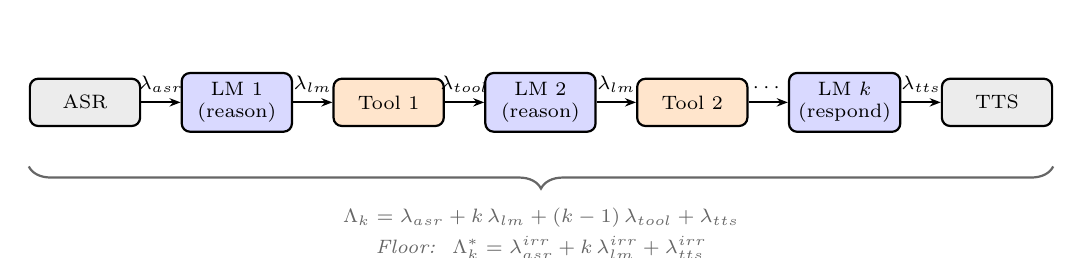
\begin{tikzpicture}[
  node distance=0.25cm and 0.5cm,
  box/.style={rectangle, rounded corners=3pt, draw=black, thick,
              minimum width=1.4cm, minimum height=0.6cm,
              font=\scriptsize, align=center},
  tool/.style={box, fill=orange!20},
  lm/.style={box, fill=blue!15},
  arr/.style={-{Stealth[length=4pt]}, thick},
  annot/.style={font=\scriptsize}
]

% Nodes (left to right)
\node[box, fill=gray!15] (asr)  {ASR};
\node[lm,  right=of asr]  (lm1)  {LM~1\\(reason)};
\node[tool, right=of lm1] (t1)   {Tool~1};
\node[lm,  right=of t1]  (lm2)  {LM~2\\(reason)};
\node[tool, right=of lm2] (t2)   {Tool~2};
\node[lm,  right=of t2]  (lmk)  {LM~$k$\\(respond)};
\node[box, fill=gray!15, right=of lmk] (tts) {TTS};

% Arrows with latency labels
\draw[arr] (asr)  -- (lm1)  node[midway, above, annot]{$\lambda_{asr}$};
\draw[arr] (lm1)  -- (t1)   node[midway, above, annot]{$\lambda_{lm}$};
\draw[arr] (t1)   -- (lm2)  node[midway, above, annot]{$\lambda_{tool}$};
\draw[arr] (lm2)  -- (t2)   node[midway, above, annot]{$\lambda_{lm}$};
\draw[arr] (t2)   -- (lmk)  node[midway, above, annot]{$\cdots$};
\draw[arr] (lmk)  -- (tts)  node[midway, above, annot]{$\lambda_{tts}$};

% Brace below showing total silence gap and irreducible floor
\draw[decorate, decoration={brace, amplitude=8pt, mirror}, thick, color=black!60]
  ([yshift=-0.5cm]asr.south west) -- ([yshift=-0.5cm]tts.south east)
  node[midway, below=0.4cm, annot, align=center]
  {$\Lambda_k = \lambda_{asr} + k\,\lambda_{lm} + (k-1)\,\lambda_{tool} + \lambda_{tts}$\\[2pt]
   \textit{Floor:}\;
   $\Lambda_k^* = \lambda_{asr}^{irr} + k\,\lambda_{lm}^{irr} + \lambda_{tts}^{irr}$};

\end{tikzpicture}
%
  }
  \caption{The $k$-step ReAct agent pipeline.
           Each reasoning step (blue) adds a full LM inference latency $\lambda_{lm}$;
           each tool call (orange) adds $\lambda_{tool}$.
           The total silence gap $\Lambda_k$ grows linearly with $k$,
           making the Cascade Competitiveness Criterion (Definition~\ref{def:ccc})
           increasingly hard to satisfy for tool-intensive agents.}
  \label{fig:react_loop}
\end{figure}

\subsection{Implications for Tool-Using Voice Agents}

Theorem~\ref{thm:react} has several important consequences for the design and deployment
of voice agents built on the ReAct paradigm \citep{yao2023react}.

\paragraph{CCC becomes harder to satisfy.}
For representative values ($\lambda_{lm} = 350$~ms, $\lambda_{tool} = 100$~ms,
$\lambda_{asr} = 350$~ms, $\lambda_{tts} = 200$~ms),
the silence gap for a two-step agent ($k = 2$) is already:
\[
  \Lambda_2 = 350 + 2(350) + 100 + 200 = 1350~\text{ms},
\]
nearly $7\times$ the human turn-taking threshold $\tau_{human} = 200$~ms
established by \citet{levinson2015timing} and \citet{stivers2009universals}.
Each additional reasoning step adds at least $\lambda_{lm} + \lambda_{tool} \approx 450$~ms
to the silence gap, pushing competitiveness further out of reach.

\paragraph{Chain-of-thought reasoning compounds the effect.}
When the agent uses chain-of-thought reasoning \citep{wei2023chainofthought},
each LM step generates a longer token sequence before producing the tool call
or response token.
This increases $\lambda_{lm}$ while improving response quality,
creating a fundamental quality--latency trade-off within each reasoning step.
The trade-off is multiplicative in $k$: an agent running $k$ reasoning steps
with chain-of-thought pays the overhead $k$ times.

\paragraph{Tool call latency is largely irreducible.}
Remote API tool calls involve a network round-trip that cannot be eliminated.
For tools requiring database queries or external service calls,
$\lambda_{tool}^{irr}$ reflects the minimum service response time,
set by physical network latency and server-side processing.
Only local, in-process tool calls have $\lambda_{tool}^{irr} \approx 0$;
real-world agents using web search, calendar, or CRM tools face positive
$\lambda_{tool}^{irr}$ values on the order of 50--200~ms per call
\citep{langgraph2024}.

\paragraph{The irreducible floor grows linearly with \texorpdfstring{$k$}{k}.}
Unlike the single-step case, where $\Lambda^* = 380$~ms in our running example,
a $k$-step agent has $\Lambda_k^* = 380 + (k-1) \cdot \lambda_{lm}^{irr}$ (assuming in-process tools).
For $k = 3$ and $\lambda_{lm}^{irr} = 100$~ms, this gives
$\Lambda_3^* = 380 + 2 \times 100 = 580$~ms,
nearly $3\times$ the human threshold.
No engineering lever can push below this floor without changing the pipeline
architecture: architectural modifications such as speculative execution or
parallel tool dispatch (discussed in Section~\ref{sec:design_levers}) address
the reducible terms but leave $\Lambda_k^*$ intact.


\section{Design Lever Taxonomy}
\label{sec:design_levers}
% §6 Design Lever Taxonomy
Having established the latency floor and its compounding behaviour for multi-step agents,
we now classify the engineering strategies used to reduce the perceived silence gap.
A key distinction emerges: some strategies reduce the irreducible floor $\Lambda^*$
(structural fixes), while others reduce only the reducible component $\lambda_i^r$
or mask the gap perceptually without changing the floor at all.

Figure~\ref{fig:design_levers} summarises the seven strategies across five dimensions:
the pipeline stage targeted, the latency component addressed, the headroom recovered,
and whether the strategy reduces $\Lambda^*$ itself.

\begin{figure}[t]
  \centering
  \resizebox{\linewidth}{!}{%
    % Fig 4: Design lever taxonomy matrix
% Seven strategies x five columns; explicit node placement to avoid foreach-tuple errors.
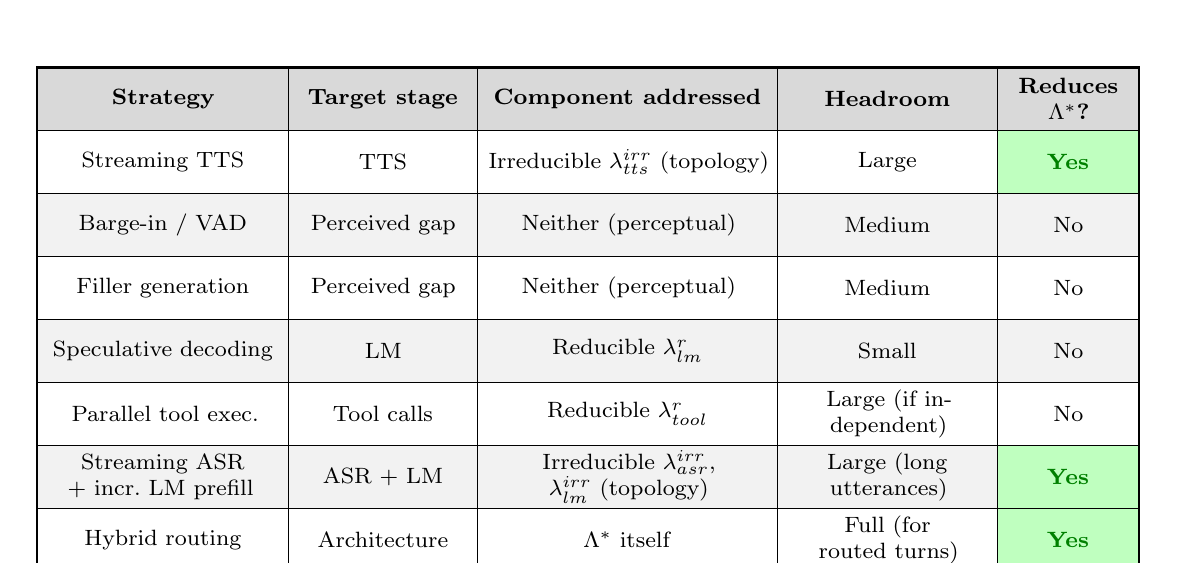
\begin{tikzpicture}[font=\footnotesize]

% Geometry (unitless numbers; appended with "cm" at each use)
\def\rh{0.80}  % row height (cm)
\def\ca{3.2}   % col 1 width: Strategy
\def\cb{2.4}   % col 2 width: Target stage
\def\cc{3.8}   % col 3 width: Component addressed
\def\cd{2.8}   % col 4 width: Headroom
\def\ce{1.8}   % col 5 width: Reduces Lambda*?

% Derived x-positions of left edges of each column
\pgfmathsetmacro{\xA}{0}
\pgfmathsetmacro{\xB}{\xA+\ca}
\pgfmathsetmacro{\xC}{\xB+\cb}
\pgfmathsetmacro{\xD}{\xC+\cc}
\pgfmathsetmacro{\xE}{\xD+\cd}
\pgfmathsetmacro{\xF}{\xE+\ce}

% Derived x-positions of centres of each column
\pgfmathsetmacro{\mA}{\xA+\ca/2}
\pgfmathsetmacro{\mB}{\xB+\cb/2}
\pgfmathsetmacro{\mC}{\xC+\cc/2}
\pgfmathsetmacro{\mD}{\xD+\cd/2}
\pgfmathsetmacro{\mE}{\xE+\ce/2}

% ── HEADER ROW (y = 0 to +\rh) ──────────────────────────────────────────────
\fill[gray!30] (\xA,0) rectangle (\xF,\rh);
\node[align=center, font=\footnotesize\bfseries, text width=\ca cm] at (\mA,{0.5*\rh}) {Strategy};
\node[align=center, font=\footnotesize\bfseries, text width=\cb cm] at (\mB,{0.5*\rh}) {Target stage};
\node[align=center, font=\footnotesize\bfseries, text width=\cc cm]
  at (\mC,{0.5*\rh}) {Component addressed};
\node[align=center, font=\footnotesize\bfseries, text width=\cd cm] at (\mD,{0.5*\rh}) {Headroom};
\node[align=center, font=\footnotesize\bfseries, text width=\ce cm]
  at (\mE,{0.5*\rh}) {Reduces $\Lambda^*$?};

% ── Helper macro: row shading ────────────────────────────────────────────────
% Row 1: y from 0 down to -\rh, row 2: -\rh to -2*\rh, etc.

% Row 1 — Streaming TTS (YES — highlighted green for last cell)
\fill[white]     (\xA,{-0*\rh}) rectangle (\xF,{-1*\rh});
\fill[green!25]  (\xE,{-0*\rh}) rectangle (\xF,{-1*\rh});
\node[align=center, text width=\ca cm]
  at (\mA,{-0.5*\rh}) {Streaming TTS};
\node[align=center, text width=\cb cm]
  at (\mB,{-0.5*\rh}) {TTS};
\node[align=center, text width=\cc cm]
  at (\mC,{-0.5*\rh}) {Irreducible $\lambda_{tts}^{irr}$ (topology)};
\node[align=center, text width=\cd cm]
  at (\mD,{-0.5*\rh}) {Large};
\node[align=center, font=\footnotesize\bfseries, color=green!50!black, text width=\ce cm]
  at (\mE,{-0.5*\rh}) {Yes};

% Row 2 — Barge-in / VAD
\fill[gray!10]   (\xA,{-1*\rh}) rectangle (\xF,{-2*\rh});
\node[align=center, text width=\ca cm]
  at (\mA,{-1.5*\rh}) {Barge-in / VAD};
\node[align=center, text width=\cb cm]
  at (\mB,{-1.5*\rh}) {Perceived gap};
\node[align=center, text width=\cc cm]
  at (\mC,{-1.5*\rh}) {Neither (perceptual)};
\node[align=center, text width=\cd cm]
  at (\mD,{-1.5*\rh}) {Medium};
\node[align=center, text width=\ce cm]
  at (\mE,{-1.5*\rh}) {No};

% Row 3 — Filler generation
\fill[white]     (\xA,{-2*\rh}) rectangle (\xF,{-3*\rh});
\node[align=center, text width=\ca cm]
  at (\mA,{-2.5*\rh}) {Filler generation};
\node[align=center, text width=\cb cm]
  at (\mB,{-2.5*\rh}) {Perceived gap};
\node[align=center, text width=\cc cm]
  at (\mC,{-2.5*\rh}) {Neither (perceptual)};
\node[align=center, text width=\cd cm]
  at (\mD,{-2.5*\rh}) {Medium};
\node[align=center, text width=\ce cm]
  at (\mE,{-2.5*\rh}) {No};

% Row 4 — Speculative decoding
\fill[gray!10]   (\xA,{-3*\rh}) rectangle (\xF,{-4*\rh});
\node[align=center, text width=\ca cm]
  at (\mA,{-3.5*\rh}) {Speculative decoding};
\node[align=center, text width=\cb cm]
  at (\mB,{-3.5*\rh}) {LM};
\node[align=center, text width=\cc cm]
  at (\mC,{-3.5*\rh}) {Reducible $\lambda_{lm}^r$};
\node[align=center, text width=\cd cm]
  at (\mD,{-3.5*\rh}) {Small};
\node[align=center, text width=\ce cm]
  at (\mE,{-3.5*\rh}) {No};

% Row 5 — Parallel tool execution
\fill[white]     (\xA,{-4*\rh}) rectangle (\xF,{-5*\rh});
\node[align=center, text width=\ca cm]
  at (\mA,{-4.5*\rh}) {Parallel tool exec.};
\node[align=center, text width=\cb cm]
  at (\mB,{-4.5*\rh}) {Tool calls};
\node[align=center, text width=\cc cm]
  at (\mC,{-4.5*\rh}) {Reducible $\lambda_{tool}^r$};
\node[align=center, text width=\cd cm]
  at (\mD,{-4.5*\rh}) {Large (if independent)};
\node[align=center, text width=\ce cm]
  at (\mE,{-4.5*\rh}) {No};

% Row 6 — Streaming ASR + Incremental LM prefill (YES — highlighted green)
\fill[gray!10]   (\xA,{-5*\rh}) rectangle (\xF,{-6*\rh});
\fill[green!25]  (\xE,{-5*\rh}) rectangle (\xF,{-6*\rh});
\node[align=center, text width=\ca cm]
  at (\mA,{-5.5*\rh}) {Streaming ASR + incr.\ LM prefill};
\node[align=center, text width=\cb cm]
  at (\mB,{-5.5*\rh}) {ASR + LM};
\node[align=center, text width=\cc cm]
  at (\mC,{-5.5*\rh}) {Irreducible $\lambda_{asr}^{irr}$, $\lambda_{lm}^{irr}$ (topology)};
\node[align=center, text width=\cd cm]
  at (\mD,{-5.5*\rh}) {Large (long utterances)};
\node[align=center, font=\footnotesize\bfseries, color=green!50!black, text width=\ce cm]
  at (\mE,{-5.5*\rh}) {Yes};

% Row 7 — Hybrid routing (YES — highlighted green)
\fill[white]     (\xA,{-6*\rh}) rectangle (\xF,{-7*\rh});
\fill[green!25]  (\xE,{-6*\rh}) rectangle (\xF,{-7*\rh});
\node[align=center, text width=\ca cm]
  at (\mA,{-6.5*\rh}) {Hybrid routing};
\node[align=center, text width=\cb cm]
  at (\mB,{-6.5*\rh}) {Architecture};
\node[align=center, text width=\cc cm]
  at (\mC,{-6.5*\rh}) {$\Lambda^*$ itself};
\node[align=center, text width=\cd cm]
  at (\mD,{-6.5*\rh}) {Full (for routed turns)};
\node[align=center, font=\footnotesize\bfseries, color=green!50!black, text width=\ce cm]
  at (\mE,{-6.5*\rh}) {Yes};

% ── GRID LINES ───────────────────────────────────────────────────────────────

% Outer border
\draw[thick] (\xA,\rh) rectangle (\xF,{-7*\rh});

% Horizontal row separators (between header and row 1, and between data rows)
\foreach \row in {0,1,2,3,4,5,6} {
  \draw (\xA,{-\row*\rh}) -- (\xF,{-\row*\rh});
}

% Vertical column separators (inner only)
\foreach \x in {\xB,\xC,\xD,\xE} {
  \draw (\x,\rh) -- (\x,{-7*\rh});
}

\end{tikzpicture}
%
  }
  \caption{Design lever taxonomy.
           Streaming TTS, streaming ASR with incremental LM prefill, and hybrid routing
           (highlighted green) reduce the irreducible latency floor $\Lambda^*$ itself.
           The remaining four strategies target reducible components or provide
           perceptual masking without structural impact on the floor.}
  \label{fig:design_levers}
\end{figure}

\subsection{Streaming Text-to-Speech}

Standard TTS systems require the complete response text before generating audio
\citep{shen2018natural}.
Streaming TTS begins audio generation after receiving a short prefix of the response ---
typically the first sentence or a fixed number of tokens.
This converts $\lambda_{tts}$ from a sequential dependency on the full LM output into
a dependency on only the first output tokens,
reducing $\lambda_{tts}^{irr}$ to the latency required to synthesise the first audio frame
from the first text tokens.
Streaming TTS therefore reduces $\Lambda^*$ directly and is a structural fix.
The tradeoff is that prosody planning across the full response is limited,
and audio quality may be lower for very short initial segments.

\subsection{Barge-In Detection}

Barge-in detection allows the agent to detect when the user begins speaking during
agent audio playback and to interrupt its own response immediately.
This does not reduce the silence gap for any individual turn where the user waits,
but it reduces the \emph{effective} silence gap by allowing the user to take the floor
before the agent has finished speaking.
Voice activity detection systems \citep{raux2008optimizing} provide the acoustic signal
for barge-in detection.
Barge-in is a perceptual patch: it masks the silence gap for turns where the user
interrupts early, but does not reduce $\Lambda^*$ for turns where the user waits for
the agent to finish.

\subsection{Filler Generation}

Filler generation plays a brief auditory cue (``hmm'', ``let me check'', ``one moment'')
immediately after ASR completes, before the LM response is ready.
This reduces the \emph{perceived} silence gap by replacing silence with an
acknowledgement signal.
Psycholinguistically, fillers signal that the conversational floor is held and
processing is underway \citep{levinson2015timing},
reducing the face-threatening interpretation of long gaps.
Filler generation does not reduce $\Lambda^*$:
the LM response must still complete before audio response begins,
and the filler audio is generated by a separate, lightweight model running in parallel
with the primary LM.
It is a perceptual patch with no structural impact on the latency floor.

\subsection{Speculative Decoding}

Speculative decoding \citep{leviathan2023fast} uses a small draft model to propose
candidate tokens that are verified in parallel by the full model,
reducing wall-clock time per generated token.
Applied to the LM stage, this reduces $\lambda_{lm}^r$ (the reducible component of LM latency)
but does not reduce $\lambda_{lm}^{irr}$,
since the prefill cost is determined by input context length
and not by token generation speed.
The practical headroom is modest: speculative decoding typically achieves 2--3$\times$
speedup on the decode phase,
with negligible effect on time-to-first-token for short responses.

\subsection{Parallel Tool Execution}

When a $k$-step ReAct agent issues tool calls that are \emph{independent} of each other
(i.e., no data dependency exists between them),
those calls can be executed in parallel rather than sequentially.
This replaces the sequential sum $(k-1) \cdot \lambda_{tool}$
with $\max_j(\lambda_{tool,j})$ in the silence gap expression,
a significant reduction for agents with many parallel-executable tool calls.
However, this strategy addresses only the reducible tool-call component;
the irreducible floor of the LM reasoning steps remains unchanged.
For tool calls with data dependencies, parallelism is not applicable.

\subsection{Streaming ASR with Incremental LM Prefill}

Streaming ASR systems---RNN-T \citep{graves2012sequence}, CTC-based streaming architectures
\citep{yao2021wenet}, and adapted Whisper variants \citep{machacek2023whisper}---emit stably
committed tokens incrementally during the user's utterance rather than buffering the complete
audio before decoding.
Coupling streaming ASR with an LM that extends its key-value cache on each committed token
converts the pipeline into a streaming cascade (Definition~\ref{def:sc}):
the LM prefill for $C_{pre}$ tokens is amortised over the user's speech duration $T_{speech}$,
reducing the post-EOU residual prefill cost to $\alpha \cdot |C_{residual}|$.

This is a \emph{structural} fix: it directly reduces $\Lambda^*$ from the EGC floor to the
streaming cascade floor of Theorem~\ref{thm:streaming_floor}:
\begin{equation}
  \Lambda^*_{SC} = \delta_N + \alpha \cdot |C_{residual}| + \lambda_{lm}^{decode,irr}
                 + \lambda_{tts}^{irr}
\end{equation}
For long utterances $|C_{residual}| \to 0$ and the saving approaches the full LM prefill cost
$\lambda_{lm}^{irr} \approx 100$~ms.
Combined with streaming TTS, the floor becomes
$\Lambda^*_{SC+sTTS} \approx \delta_N + \lambda_{lm}^{decode,irr} \approx 170$--340~ms,
competitive with buffer-and-commit native voice models (320--500~ms) while retaining all
cascade structural advantages: tool use, content moderation at the text layer, auditability,
and lower cost.

The primary engineering challenge is KV cache invalidation: when the streaming ASR revises a
token at position $k$, all cached entries at positions $k, k+1, \ldots$ are stale and must be
recomputed at cost $\alpha \cdot (|C_{pre}| - k)$ \citep{xiao2023streamingllm}.
The stability-latency tradeoff of streaming ASR---the fraction of tokens that survive to the
final hypothesis without revision, as a function of lookahead depth---is formally characterised
by \citet{selfridge2011stability}.
Revision frequency depends on the ASR architecture; streaming RNN-T systems
\citep{sainath2020streaming} exhibit commit latencies of 150--320~ms with low revision rates,
making them the most suitable pairing for incremental LM prefill.
The accuracy-latency tradeoff of $\delta_N$ is characterised as an open problem in
Section~\ref{sec:open_problems}.

\subsection{Hybrid Routing}

Hybrid routing dispatches conversational turns to either a cascade pipeline or a native
voice model based on predicted turn complexity \citep{dong2024building}.
Simple turns --- factual questions, short responses, no tool use expected ---
are routed to the cascade pipeline, which is cheaper and more auditable.
Complex turns that require multi-step tool use or long responses may be routed to a
native voice model.
When a turn is handled by the native model, its silence gap replaces the cascade gap
entirely, effectively reducing $\Lambda^*$ to the native model's irreducible floor
for that turn.
Hybrid routing is therefore the only strategy that can eliminate the cascade latency
floor entirely, albeit only for selected turns.
The tradeoffs are cost (native model API calls are more expensive),
integration complexity (two parallel pipelines must be maintained),
and routing accuracy (misclassification sends tool-intensive turns to a pipeline
that cannot support them).

\subsection{Summary}

Three strategies reduce $\Lambda^*$ structurally: streaming TTS, streaming ASR with
incremental LM prefill, and hybrid routing.
The remaining four strategies reduce only reducible components or provide perceptual masking.

Streaming TTS should be the first modification applied to any cascade voice system:
it requires no architectural change and provides the largest structural headroom reduction
at low engineering cost.
Streaming ASR with incremental LM prefill should be the second: combined with streaming TTS
it yields a floor of 220--440~ms for typical utterances, placing the pipeline within the
range of buffer-and-commit native voice models while retaining cascade structural advantages.
Hybrid routing should be considered when the streaming cascade floor is still insufficient
to satisfy the CCC and the use case includes a meaningful fraction of simple turns.
The remaining four strategies are valuable complements but cannot, alone or in combination,
bring a cascade pipeline below its structural latency floor.


\section{Open Problems}
\label{sec:open_problems}
% §7 Open Problems
Our formal analysis reveals several open research directions that go beyond the scope of this paper.

\paragraph{Learned barge-in prediction.}
Current barge-in systems react to voice activity after it begins.
A predictive system would detect \emph{intent to speak} from prosodic cues (rising pitch, trailing cadence, filled pause) before the user actually starts speaking.
The agent can then pre-emptively silence its response.
This would effectively reduce the perceptual silence gap for interruption turns below zero---the agent stops before the user begins.
Formalising the prediction problem and establishing the tradeoff between false-positive barge-in rate and turn-taking smoothness is an open problem.

\paragraph{Safety in cascade voice systems.}
The cascade architecture introduces safety risks at each inter-component boundary.
ASR transcription errors can transform benign speech into harmful text inputs.
TTS injection attacks could exploit the text interface of the TTS component to produce audio content not intended by the LM.
Voice-channel jailbreaks may exploit prosodic or phonetic properties of the audio input that are discarded by ASR transcription.
A formal threat model for cascade voice systems, analogous to the text-based guardrail frameworks of \citet{dong2024building}, does not yet exist.

\paragraph{Voice-aware agent planning.}
The ReAct agent in our model is latency-unaware.
It selects tool calls and reasoning depth based solely on task requirements.
A voice-aware agent would reason about its remaining silence budget ($\tau_{human} - \Lambda_{\text{elapsed}}$) as a first-class planning constraint.
It would prefer shallower reasoning chains and pre-cached tool results when the budget is nearly exhausted.
Formalising this as a constrained planning problem and studying the quality-latency tradeoff it induces is an open direction.

\paragraph{Principled hybrid routing policies.}
Hybrid routing (Section~\ref{sec:design_levers}) requires a policy for classifying incoming turns as simple (cascade-suitable) or complex (native-suitable).
No principled approach to learning this routing policy currently exists.
Key challenges include defining the optimal routing objective (minimise cost subject to CCC satisfaction, or maximise quality subject to budget).
Handling turns that are initially classified as simple but escalate (the LM discovers mid-reasoning that a tool call is needed) is a further challenge.
Maintaining conversational context across pipeline switches (the native model and the cascade LM have different context representations) remains open.

\paragraph{Commit latency--accuracy Pareto frontier for streaming ASR.}
Theorem~\ref{thm:streaming_floor} shows that the streaming cascade floor $\Lambda^*_{SC}$
is dominated by the ASR commit latency $\delta_N$.
Reducing $\delta_N$ below 100~ms---the threshold at which the CCC becomes satisfiable
(Corollary~\ref{cor:streaming_ccc})---requires increasing the lookahead depth of the ASR
model, which decreases word error rate at the cost of increased $\delta_N$, or decreasing
lookahead, which reduces $\delta_N$ at the cost of higher WER.
No published work characterises this Pareto frontier for modern neural streaming ASR systems
paired with LLM-scale language models.
Formalising the tradeoff as a constrained optimisation---minimise expected $\delta_N$ subject
to a WER budget---and studying the optimal operating point across utterance types and domains
is an open problem with direct engineering impact.

\paragraph{Speculative cascade: early generation on partial transcripts.}
A natural extension of streaming ASR is to begin LM \emph{generation} (not just prefill)
on the stable ASR prefix before EOU is confirmed---analogously to speculative decoding
\citep{leviathan2023fast} but at the ASR hypothesis level.
Let $p_{accept}$ be the probability that the ASR does not revise any token that changes the
semantics of the LM's first response token.
The expected silence gap is:
\begin{equation}
  \mathbb{E}[\Lambda_{spec}] = p_{accept} \cdot \Lambda_{early}
    + (1 - p_{accept}) \cdot (\Lambda^*_{SC} + \lambda_{replan})
\end{equation}
Deriving $p_{accept}$ as a function of ASR model type and query distribution,
bounding the replan cost $\lambda_{replan}$,
and characterising the quality degradation from incorrect speculative generation
(especially when TTS has already begun audio playback from the wrong draft) are open problems.
The SDS literature \citep{schlangen2011general} treats revocability informally;
a formal quantitative treatment for transformer LM--streaming ASR pairs does not yet exist.

\paragraph{Probabilistic EOU detection as a design lever.}
Current EOU detection is reactive: the VAD window $d_{eou}$ is a fixed silence threshold.
Prosodic and syntactic predictors can estimate $P(\text{EOU} \mid \text{acoustic features},
C_{pre})$ before acoustic silence begins, triggering LM generation when this probability
exceeds a threshold $\theta$.
This converts $d_{eou}$ from a deterministic floor to a stochastic variable:
$d_{eou}(\theta) = \mathbb{E}[\text{anticipation horizon}] - P_{fal}(\theta) \cdot \lambda_{restart}$,
where $P_{fal}(\theta)$ is the false-EOU rate and $\lambda_{restart}$ is the cost of
restarting after a false trigger.
Characterising the optimal $\theta$ that minimises expected $\Lambda^*_{SC}$ subject to
a tolerable false-EOU rate, and establishing a revised impossibility condition when
$d_{eou}$ is treated as a stochastic design variable, is an open formal problem.


\section{Discussion}
\label{sec:discussion}
% §8 Discussion
\subsection{Practitioner Guidance}

Our analysis yields concrete guidance for teams building cascade voice agents.

\paragraph{When cascade is sufficient.}
A cascade agent without tool use ($k=0$) with streaming TTS can achieve a silence gap as low as $\Lambda^* \approx 280$~ms (using representative values from Table~\ref{tab:latency_example} with $\lambda_{tts}^{irr}$ reduced to 0 by full streaming).
This is close to but not within the 200~ms threshold.
For applications where users tolerate slightly longer gaps (e.g., task-oriented dialogue where cognitive load reduces gap sensitivity), a streaming-TTS cascade is a reasonable choice.

\paragraph{When tool use is required.}
For $k \geq 1$, the silence gap grows by at least $\lambda_{lm}^{irr} \approx 100$~ms per step.
Filler generation is strongly recommended for any tool-using cascade agent to mask the silence gap perceptually.
Parallel tool execution should be implemented wherever tool calls are independent.
For $k \geq 3$, the irreducible floor exceeds 500~ms regardless of optimisations.
Users will perceive the delay as significant.
In these cases, hybrid routing to a native voice model for tool-intensive turns is the only structural solution.

\paragraph{When to choose native voice.}
Native voice models are justified in three cases.
First, the CCC cannot be satisfied by any combination of the structural levers (streaming TTS and hybrid routing).
Second, the turn mix is dominated by short, conversational turns where the overhead of the cascade pipeline is felt most acutely.
Third, barge-in and interruption handling quality is a hard requirement, since native models handle these natively without a separate VAD pipeline.
The higher cost and reduced auditability of native models are the primary tradeoffs.

\subsection{Limitations}

The perceptual threshold $\tau_{human} = 200$~ms is derived from studies of natural human-human conversation \citep{levinson2015timing,stivers2009universals}.
Human-agent interaction may have different norms.
Users may calibrate expectations downward when they know they are speaking to an AI.
Our analysis treats $\tau_{human}$ as a constant, but future work should treat it as a distribution conditioned on user, context, and task type.

The latency decomposition in Definition~\ref{def:decomposition} assumes that irreducible latencies are stable across inputs.
In practice, $\lambda_{lm}^{irr}$ grows with context length, and $\lambda_{asr}^{irr}$ grows with utterance complexity.
A more complete model would express irreducible latencies as functions of input characteristics.

Our model does not account for network latency between pipeline components, which adds a reducible but non-negligible contribution in cloud-hosted deployments.


\section{Conclusion}
\label{sec:conclusion}
% §9 Conclusion
We have presented the first formal characterisation of the irreducible latency floor as a function of cascade pipeline topology, together with formal conditions for perceptual competitiveness with native voice models.
While the spoken dialogue systems literature \citep{schlangen2011general,skantze2021turn} motivates streaming as an engineering solution to sequential latency accumulation, our work is the first to derive a formal lower bound on the irreducible floor and to connect it explicitly to the Cascade Competitiveness Criterion and multi-step tool-using agents.
Our Latency Floor Theorem (Theorem~\ref{thm:latency_floor}) establishes that the silence gap of any cascade pipeline has an irreducible lower bound $\Lambda^*$, the sum of irreducible per-stage latencies, that cannot be reduced by model improvements or hardware upgrades alone.
The Cascade Competitiveness Criterion (Definition~\ref{def:ccc}) identifies the formal condition---$\Lambda \leq \tau_{human}$---under which a cascade agent achieves perceptual equivalence with a native voice model.
For representative current systems, $\Lambda^* > \tau_{human}$, establishing an impossibility result (Corollary~\ref{cor:impossibility}): no standard cascade pipeline can be perceptually competitive in the strict sense.

We extended the model to tool-using ReAct agents (Theorem~\ref{thm:react}) and proved that each reasoning step adds a full LM inference cycle to the irreducible floor, making CCC satisfaction increasingly unlikely for multi-step agents.
Our design lever taxonomy classifies six engineering strategies by their structural impact: only streaming TTS and hybrid routing reduce $\Lambda^*$ itself; the remaining four are perceptual patches.

Together, these results give practitioners a principled basis for architecture selection and system optimisation, and identify four open research directions: learned barge-in prediction, safety in cascade voice systems, voice-aware agent planning, and principled hybrid routing policies.
As voice interfaces become a primary modality for human-AI interaction, formal understanding of their latency structure will be essential for designing systems that meet human conversational expectations.


\bibliographystyle{plainnat}
\bibliography{main}

\end{document}
